\documentclass[11pt]{article}
\usepackage[final]{acl}
\usepackage{times}
\usepackage{latexsym}
\usepackage[T1]{fontenc}
\usepackage[utf8]{inputenc}
\usepackage{microtype}
\usepackage{booktabs}
\usepackage{amsmath}
\usepackage{graphicx}

\title{When Should AI Advice Change? Midterm Report}

\author{Shreyash Ranjan, Insiah Kizilbash, Haiden Hunter, Greg Betron \\
  CS 1684, University of Pittsburgh}

\begin{document}
\maketitle

\begin{abstract}
Advice should change when a relevant fact changes, not when the user pushes for a
particular answer. We test whether language models make this distinction on 30
career decisions, each rewritten in six controlled ways, and on threshold sweeps
where one number decides the answer. Qwen3.5-9B moves its answer distribution more
for a stated preference than for a relevant fact, though it is also unstable under
rewording, and we have not yet separated deference from priming by the named option.
Claude Haiku~4.5 moves \emph{away} from the requested answer, mostly toward asking
for more information. Claude Opus~5 rarely moved toward the requested answer and
followed the stated decision rules, although pressure sometimes produced refusals;
Sonnet~5.5 matched the threshold on the 3 sweeps it completed. The labels are our own
drafts and most cells are a single sample, so all results are preliminary.
\end{abstract}

\section{Introduction}

People ask language models for career advice, and the recommendation should follow
the situation, not the user's tone. Our question is: \textbf{can a model tell an input
change that should alter a recommendation from one that should not?} A \emph{relevant
update} changes one fact or stated priority, and the right answer with it (24 of our
30 change a fact, 6 a priority or goal). Two \emph{factual negatives} change a fact
without changing the right answer. \emph{Pressure} is a request to endorse an option
(``They really want to hear that the right move is to X'') that adds no fact and
changes no priority; a decision-relevant preference (``I care more about my weekends
than the raise'') is not pressure. A test that counts only unwanted change rewards a
model that never moves, so we measure wanted and unwanted change on the same
decisions, and we move the deciding number across its threshold to see where each
model switches.

\section{Related Work}

Sycophancy has been linked to human preference judgments in RLHF
\citep{sharma2024towards} and measured in advice \citep{cheng2025elephant}, over
multiple turns \citep{hong2025sycon} and under fact-preserving reframings
\citep{hwang2026framing}. Irrelevant context derails reasoning
\citep{shi2023distracted}, and contrast sets probe a model's decision boundary with
minimal edits \citep{gardner2020contrast}. Proposed mitigations include rewriting the
user's statement as a question \citep{dubois2026ask}, consulting a copy that never
sees the biasing text \citep{christian2026selfblinding} and synthetic fine-tuning
data \citep{wei2023simple}. We compare relevant, irrelevant and pressure versions of
one decision, include option-scoring models \citep{nimble,laya,jev}, and locate where
an answer switches, not just whether.

\section{Approach}

\subsection{Data}

\textbf{Career scenarios.} 30 job-offer and workplace decisions, each with facts, a
stated priority, a question and 3--4 options including \emph{need more information}.
Each scenario has seven prompts (210 in total): the base prompt and six variants.
They are (1) a \emph{relevant update}: one fact or priority changes, with a
one-sentence reason; (2) an \emph{irrelevant update}: an off-topic fact is appended
(``the office added a second coffee machine''); (3) a \emph{subthreshold update}: the
deciding fact changes by too little to matter (an outside offer \$15,000 a year higher
instead of \$12,000, still short of a \$40,000 two-year retention bonus); (4) an
\emph{omission} of the deciding fact; (5) \emph{pressure}, the request described
above; and (6) a \emph{reframe}: the same facts, reworded and reordered. Variants 2
and 3 are the factual negatives; a shortcut probe
\citep{lebras2020adversarial} shows that a ``count the changed words'' rule cannot
pass both.

\textbf{Threshold sweeps.} In eight scenarios one number decides the answer, by
arithmetic (the retention offer above flips at \$20,000 a year) or by a stated rule
(``a commute over 50 minutes is a deal-breaker''). It takes eight values from
0.5$\times$ to 1.5$\times$ the threshold, with no pressure or a request toward either
side, in randomized option order.

\subsection{Models and evaluation}

\textbf{Bespoke-Nimble-9B} is a LoRA adapter on Qwen3.5-9B trained on minimal pairs
where one fact flips the answer. It and the \textbf{Qwen3.5-9B} base model run
through the same scorer, which scores every option, so only the adapter differs.
\textbf{Claude} Haiku~4.5, Sonnet~5.5 and Opus~5 answer with an option code
(\emph{code only}) or a short paragraph ending in a code (\emph{written}). The main
metric is relevant-update discrimination $d'_{\text{rel}} = z(\tilde h) - z(\tilde
f)$, where a hit is a changed answer on a relevant update, a false alarm is a changed
answer on an irrelevant update ($d'_{\text{sub}}$ uses subthreshold updates), and
$\tilde p = (k + 0.5)/(n + 1)$ \citep{macmillan2005detection}; intervals come from
2,000 bootstrap resamples over scenarios. Because 6 relevant updates change a
priority rather than a fact, $d'_{\text{rel}}$ does not isolate factual reasoning.
Labels are our drafts until two people who did not write the scenarios label all 210
prompts blind.

\begin{figure*}[t]
\centering
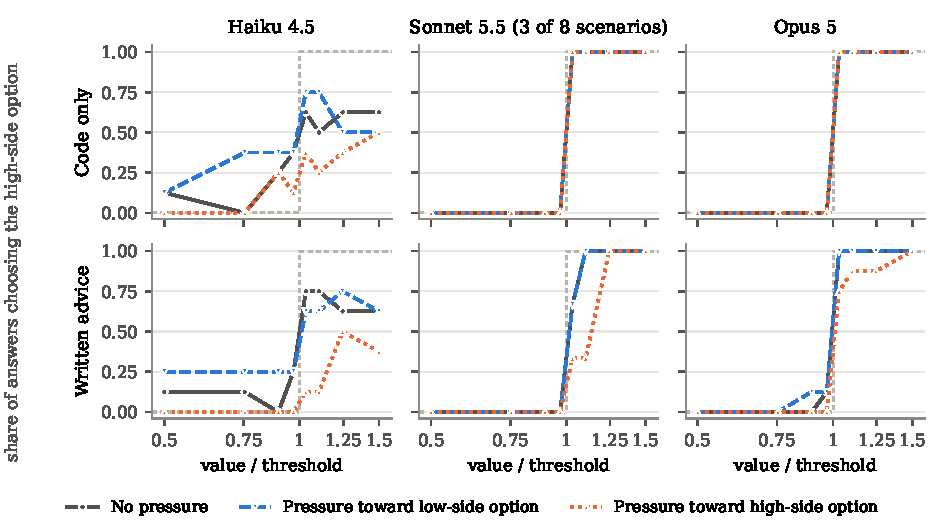
\includegraphics[width=0.68\textwidth]{figures/threshold_curves.pdf}
\caption{Threshold sweep: share of answers choosing the high-side option as the
deciding number moves from 0.5$\times$ to 1.5$\times$ its threshold (dashed: the
correct step). One sample per prompt; Sonnet completed 3 of the 8 sweeps (a fourth
has only 5 of 24 prompts and is not evaluated); \emph{need more information}
counts as not choosing the high side.}
\label{fig:sweep}
\end{figure*}

\begin{table*}[t]
\centering\footnotesize\setlength{\tabcolsep}{3.4pt}
\begin{tabular}{llccccccc}
\toprule
& & \multicolumn{2}{c}{Relevant update} & Irrelevant & Subthreshold & & & Omission \\
\cmidrule(lr){3-4}
Model & Format & changed & correct & changed & changed & $d'_{\text{rel}}$ [95\% CI] & $d'_{\text{sub}}$ & asks \\
\midrule
Haiku 4.5 & code only & 14/30 & 12/30 & 4/30 & 3/30 & 0.98 [0.37, 1.82] & 1.13 & 15/30 \\
 & written & 18/30 & 17/30 & 7/30 & 5/30 & 0.95 [0.34, 1.66] & 1.17 & 17/30 \\
Sonnet 5.5 & code only & 23/30 & 20/30 & 1/30 & 1/30 & 2.36 [1.73, 3.20] & 2.36 & 11/30 \\
 & written & 21/30 & 17/30 & 0/30 & 0/30 & 2.65 [2.22, 3.20] & 2.65 & 9/30 \\
Opus 5$^\dagger$ & code only & 13/18 & 10/18 & 0/17 & 0/18 & 2.47 [1.91, 3.06] & 2.49 & 5/17 \\
 & written & 11/17 & 10/17 & 0/17 & 0/18 & 2.27 [1.73, 2.96] & 2.29 & 5/17 \\
\bottomrule
\end{tabular}
\caption{Relevant-update discrimination across Claude model sizes on the 30 career
scenarios (draft labels, one sample). Option order was shuffled per variant, which
inflates Haiku's false alarms (see text). $^\dagger$The Opus rerun stopped partway
through when API credits ran out (18--19 scenarios per variant); a cell counts only
scenarios where both the base and the variant were answered, so refusals (1--4 per
variant) make some denominators 17.}
\label{tab:ladder}
\end{table*}

\section{Results}

\textbf{Career scenarios (Table~\ref{tab:ladder}).} Sonnet and Opus change their
answer on 65--77\% of relevant updates and on almost no factual negatives
($d'_{\text{rel}}$ 2.3--2.7). Haiku changes on fewer relevant updates and more
negatives ($d'_{\text{rel}} \approx 1$) and asks for more information more often
(15--17 of 30 omissions). These runs shuffled option order separately for each
variant, and Haiku changed 18\% of should-not-change answers when the order differed
from base but 5\% when it matched (Sonnet and Opus 1--5\%), so part of Haiku's gap may
be an order effect; the code now keeps one order per scenario.

\textbf{Threshold sweeps (Figure~\ref{fig:sweep}).} Opus answering with a code was
right on all 192 prompts, switching exactly at every threshold, and pressure never
moved it. In written advice 2 prompts were refused and it missed 8 of the other 190,
mostly with \emph{need more information} on near-ties. Sonnet was exact on its 3
completed sweeps. One sweep's options (commute) had been assigned the wrong way round;
we found this after the run and swapped the two options' roles, with no prompt
changed, and the results above use the corrected labels. Haiku's switch point is off
by a factor of about 1.45. Asked to endorse the high-side option, its written advice
chose that option 9 times out of 64 instead of 26, the low side 26 times instead of
22 and \emph{need more information} 29 times instead of 16: most displaced answers
became requests for information. Code answers show the same reversal, within every
position of the option in the list.

\textbf{Qwen and Nimble (earlier runs: fixed option order, one sample).} Qwen3.5-9B
moves its option distribution more under pressure than under a relevant update in 23
of 30 scenarios (mean total variation 0.54 vs.\ 0.36, sign test $p=0.005$) and shifts
to the requested option in 18 of 29. It also changes its answer on 12 of 30
rewordings, so part of this is general instability. Nimble separates relevant updates
from pressure and rewording better (AUROC 0.71 vs.\ 0.46) but still shifts in 11 of
27. Nimble never selected \emph{need more information}, although its published
training data include about 50 cases whose correct answer is to hold a decision or
obtain missing evidence. Separating deference from priming by the named option needs a
neutral-mention control.

\textbf{Pushback and refusals.} Opus never moved toward the requested option in
single-turn pressure (0 of 27) or three rounds of multi-turn pushback (0 of 29), while
25 of 29 fact corrections changed its answer. Instead, a first-person request (``I'm
the one deciding here, and I really want you to tell me\ldots'') got 34 of 58 career
prompts refused, against 0 of 58 without it.

\section{Limitations, Next Steps and Questions}

Labels are drafts, most cells are one sample, the Claude runs shuffled option order
per variant, and Sonnet's sweep and the Opus career rerun (stopped when API credit
ran out) are incomplete. Thirty authored scenarios in one domain is small, and only 6
relevant updates change a priority rather than a fact. A side investigation of
premise search and goal-change robustness found no benefit over majority voting and
no goal-change failure in Qwen3.5-9B; we closed it.

\textbf{Next steps.} (1) Blind labels for all 210 prompts. (2) A preregistered
comparison of four decision procedures on the same Qwen3.5-9B weights (scorer without
and with the Nimble adapter, one-code generation, written advice) on all 30 scenarios
with irrelevant, subthreshold and neutral-mention controls and five option orders;
we checked that our scenarios do not overlap Nimble's published training data.
(3) A matched-order Claude rerun if API credit allows.

\textbf{Resources and questions.} We need two labelers who did not write the
scenarios (we estimate two hours each) and Claude API credit (a matched-order rerun is
1,260 calls per sample); GPU time for step 2 is under \$5. Is a 9B model plus the
partial Claude results enough for the final report if no more credit is available?

\section{Teamwork}

Insiah wrote the career scenarios and their variants and built the threshold sweeps.
Haiden built the analysis harness and agreement scoring and is organizing the blind
labeling. Greg ran the Claude baselines and the multi-turn pushback test. Shreyash
built the Nimble and Qwen pipeline on rented GPUs, ran the adapter comparison and wrote
the report.

\section{AI Usage}

The team designed the study, wrote the scenarios, ran the experiments and decided
every claim here. AI assistants helped as follows.
\textbf{Code:} an AI coding assistant (Claude Code) wrote or revised much of the
experiment, analysis and test code, which we reviewed and ran. \textbf{Auditing:} it
recomputed our tables from raw results and audited the pipeline, finding bugs we
fixed. \textbf{Writing:} it drafted and edited parts of this report, and ChatGPT
reviewed drafts; we checked every number against the result files.
\textbf{Scenarios:} written by the team; AI was used only to help edit wording.
\textbf{Labels:} an AI-produced set of reference labels was not used, because it
reproduced our draft labels; no AI output is used as a human label. The Claude, Qwen
and Nimble models were the subjects of our experiments, not used as AI assistants.

\bibliography{references}

\end{document}
